\documentclass[../../../../main.tex]{subfiles}
\begin{document}

\begin{flushright}
\footnotesize\textit{【自動文字起こし・要確認】}
\end{flushright}

\noindent
[\textbf{解}] $X = \sqrt{x}, Y = \sqrt{y}$ とおくと，
\[
X \geqq 0, \quad Y \geqq 0, \quad X^2 + Y^2 \geqq 1 \quad \dots \text{①}
\]
の時，$g(X, Y) = X + aY$ の $\min$ をもとめればよい。$k = X + aY \dots \text{②}$ とおいて，$Y$-$X$ 平面で ①, ②が交点を持つ条件をもとめればよい。

\begin{enumerate}
    \item[$1^\circ$] $0 < a \leqq 1$ の時\\
    ②が $(Y, X) = (1, 0)$ を通る時で，$\min k = a$
    \item[$2^\circ$] $a \geqq 1$ の時\\
    ②が $(Y, X) = (0, 1)$ を通る時で，$\min k = 1$
\end{enumerate}

\noindent
従って，
\[
\min f(x, y) = \min \{a, 1\}
\]
である。

\begin{center}
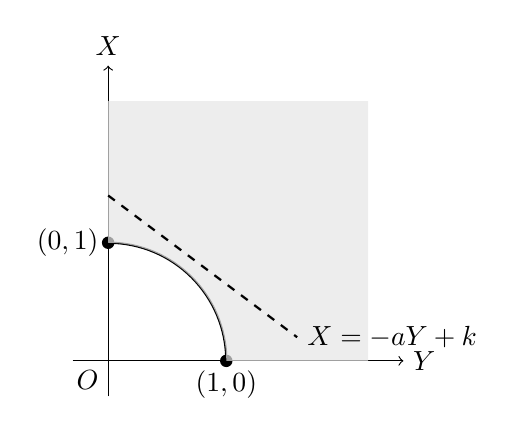
\begin{tikzpicture}[scale=1.5]
    \draw[->] (-0.3,0) -- (2.5,0) node[right]{$Y$};
    \draw[->] (0,-0.3) -- (0,2.5) node[above]{$X$};
    \node[below left] at (0,0) {$O$};

    % Quarter circle
    \draw[thick] (1,0) arc (0:90:1);
    \fill (1,0) circle (1.5pt) node[below]{$(1,0)$};
    \fill (0,1) circle (1.5pt) node[left]{$(0,1)$};

    % Hatching region X^2+Y^2 >= 1, X>=0, Y>=0
    \fill[gray!20, opacity=0.7] (1,0) arc (0:90:1) -- (0,2.2) -- (2.2,2.2) -- (2.2,0) -- cycle;

    % Line X = -aY + k
    \draw[thick, dashed] (0, 1.4) -- (1.6, 0.2) node[right]{$X = -aY + k$};
\end{tikzpicture}
\end{center}

\vspace{1em}
\noindent
[\textbf{解} \quad 一応，上が一番早い気がしただけで本流もある]

\vspace{0.5em}
\noindent
$f(x, y) = \sqrt{x} + a\sqrt{y}$ において $x$ を固定する。$a > 0$ に注意して
\[
\begin{aligned}
\min f(x, y) &= \sqrt{x} + a\sqrt{1-x} \quad (0 \leqq x \leqq 1) \quad \dots \text{①} \\
\min f(x, y) &= \sqrt{x} \quad (1 \leqq x) \quad \dots \text{②}
\end{aligned}
\]
①の時，$x$ をうごかして，$\min f(x, y) = \min \{a, 1\}$\\
②の時 \quad $\prime\prime$ \quad $\min f(x, y) = 1$

\vspace{0.5em}
\noindent
したがって
\[
\min f(x, y) = \min \{a, 1\}
\]

\end{document}
